% ----------------------------------------------------------
\chapter{Algoritmos e estruturas de dados para consulta de pontos no plano}\label{cap:desenvolvimento}
% ----------------------------------------------------------
Nesta seção veremos formas de construir estruturas de dados para um conjunto de pontos no plano. 
Consideramos que os pontos são fixos. Para cada estrutura construída, veremos também como utilizá-la para
consultar pontos dentro de uma janela.

% ----------------------------------------------------------
\section{Árvore KD}
% ----------------------------------------------------------

Uma árvore KD é uma árvore binária onde cada folha é um ponto \textit{k-dimensional}.
Cada nó não-folha guarda um valor $v$ em uma dimensão $d$.
Pontos cujo os valores na dimensão $d$ são iguais ou menores a $v$ estão na subárvore à esquerda,
e respectivamente, pontos com valores na dimensão $d$ na subárvore à direita.
Cada nível da árvore é associado a uma das \textit{k dimensões}. Então, a citar um exemplo no plano,
se dado nível considera o eixo $x$, a subárvore à esquerda contém os pontos com o eixo $x$ menor que o valor 
$v$. Similarmente, à direita contém os pontos com o eixo $x$ maior que o valor $v$.

\subsection{Árvore 2D}
Uma árvore 2D é a versão com duas dimensões para árvores KD. A sua construção considera um dado conjunto 
de pontos no plano ($P$) e pode ser feita da seguinte forma. Na construção de uma árvore para 2 dimensões,
cada ponto tem uma forma $p = (p_x, p_y)$ . Escolhemos um eixo para iniciar a construção da árvore.
Ao iniciar a construção, realizamos uma $x$-ordenação e uma $y$-ordenação nos pontos de $P$
(no caso $n$ dimensional, faremos $n$-ordenações). Chamaremos o conjunto de pontos ordenados pelo eixo
$x$ de $P_{ord(x)}$, e ordenados por $y$ de $P_{ord(y)}$.

Fixado um eixo, o valor da mediana dos pontos ordenados neste eixo será o valor $v$ escolhido para dividir
$P$ em dois subconjuntos, e serão criados dois subconjuntos.\cite{cg08}.Chama-se recursivamente a
construção das subárvores à esquerda e à direita de $v$ alternando o eixo e passando os subconjuntos.
Considere o seguinte conjunto de pontos.

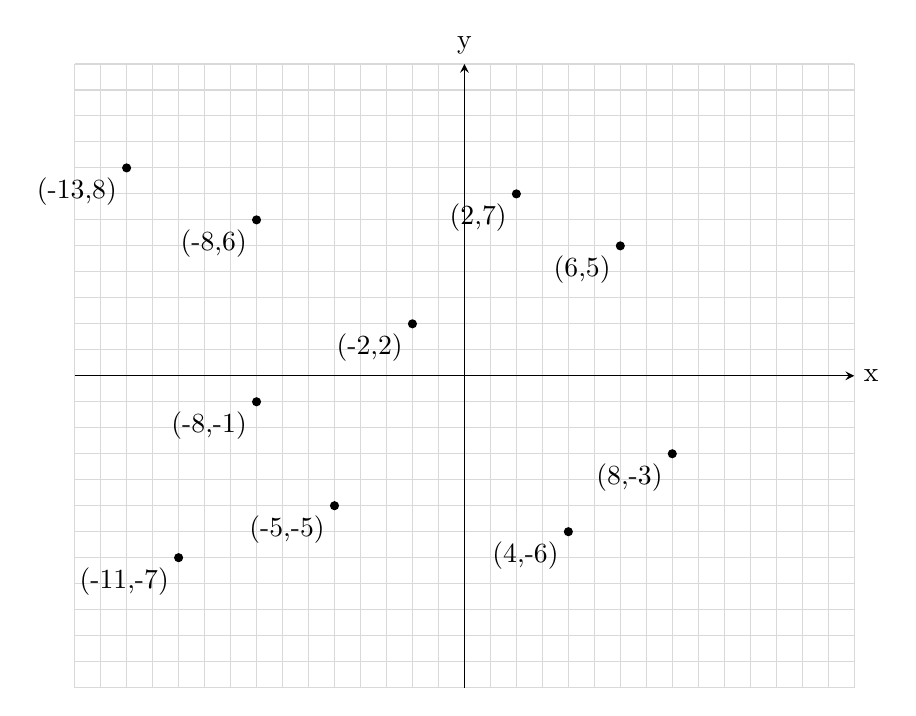
\begin{tikzpicture}[scale=0.33]
  \draw[gray!30] (-15,-12) grid[xstep=1, ystep=1]  (15,12);
  \draw[-stealth] (-15,0)--(15,0) node[right]{x}; % x axis
  \draw[-stealth] (0,-12)--(0,12) node[above]{y}; % y axis


  \fill (-13,8)  circle[radius=5pt] node[anchor=north east]{(-13,8)};
  \fill (-8,6)  circle[radius=5pt] node[anchor=north east]{(-8,6)};
  \fill (-2,2)  circle[radius=5pt] node[anchor=north east]{(-2,2)};
  \fill (-8,-1)  circle[radius=5pt] node[anchor=north east]{(-8,-1)};
  \fill (-11, -7)  circle[radius=5pt] node[anchor=north east]{(-11,-7)};
  \fill (-5,-5)  circle[radius=5pt] node[anchor=north east]{(-5,-5)};
  \fill (2,7)  circle[radius=5pt] node[anchor=north east]{(2,7)};
  \fill (6,5)  circle[radius=5pt] node[anchor=north east]{(6,5)};
  \fill (8,-3)  circle[radius=5pt] node[anchor=north east]{(8,-3)};
  \fill (4,-6)  circle[radius=5pt] node[anchor=north east]{(4,-6)};
\end{tikzpicture}


Inicialmente escolhemos o eixo $x$. Acompanharemos a troca de eixos de acordo com o nível da árvore.
Caso o nível seja $par$, consideramos o eixo $x$, do contrário, eixo $y$.
Como temos $P_{ord(x)}$, sabemos que o ponto médio representará o valor $x_{mediana}$.
Criamos dois subconjuntos $P_1$ e $P_2$ tal que:

    $P_1 = \{p \in P : p_x \leq x_{mediana}\}$ e $P_2 = \{p \in P : p_x > x_{mediana}\}$.

Agora, recursivamente, repete-se para os dois novos conjuntos criados considerando o eixo $y$ e 
continua da mesma forma até restar somente um ponto. Este, por sua vez, será um nó folha da árvore e
tratado na base da recursão do algoritmo. A árvore 2D correspondente à figura anterior e o pseudocódigo
para a construção de uma árvore 2D são dados em seguida.


\begin{algorithm}
    \caption{O algorítimo \Call{ConstroiArvore2D}{$P$, $profundidade=0$}, recebe um conjunto de 
    pontos $P$ no plano e uma profundidade da árvore.
    O algoritmo devolve a raiz de uma árvore 2D.}
    \begin{algorithmic}[1]
        \Function{ConstróiÁrvore2D}{$P$, $profundidade$}
            \If{P contém apenas um ponto}
            \Return $nó \leftarrow ponto$
        \Else
            \If{$profundidade$ é par}
            \State 
                Divide P em dois subconjuntos pela mediana $l$ da $x$-coordenada dos pontos \newline
                \hspace*{5em}em P. Seja $P_1$ o conjunto dos pontos à esquerda de $l$ e seja $P_2$
                \hspace*{5em} o conjunto de pontos à direita de $l$.
            \Else
            \State
                Divide P em dois subconjuntos com um pela mediana $l$ da $y$-coordenada dos pontos em P.
                Seja $P_1$ o conjunto dos pontos abaixo de $l$ e seja $P_2$ o conjunto de pontos acima de $l$.
            \EndIf
        \EndIf
        \State Cria os nós $v_{esquerda}$ e $v_{direita}$
        \State $v_{esquerda} \leftarrow $ \Call{ConstróiÁrvore2D}{$P_1, profundidade+1$}
        \State $v_{direita} \leftarrow $ \Call{ConstróiÁrvore2D}{$P_2, profundidade+1$}
        \State Cria um nó $v$, associamos o valor $l$ e associamos os filhos $v_{esquerda}$ e $v_{direita}$ 

        \Return $v$
        \EndFunction
    \end{algorithmic}
\end{algorithm}

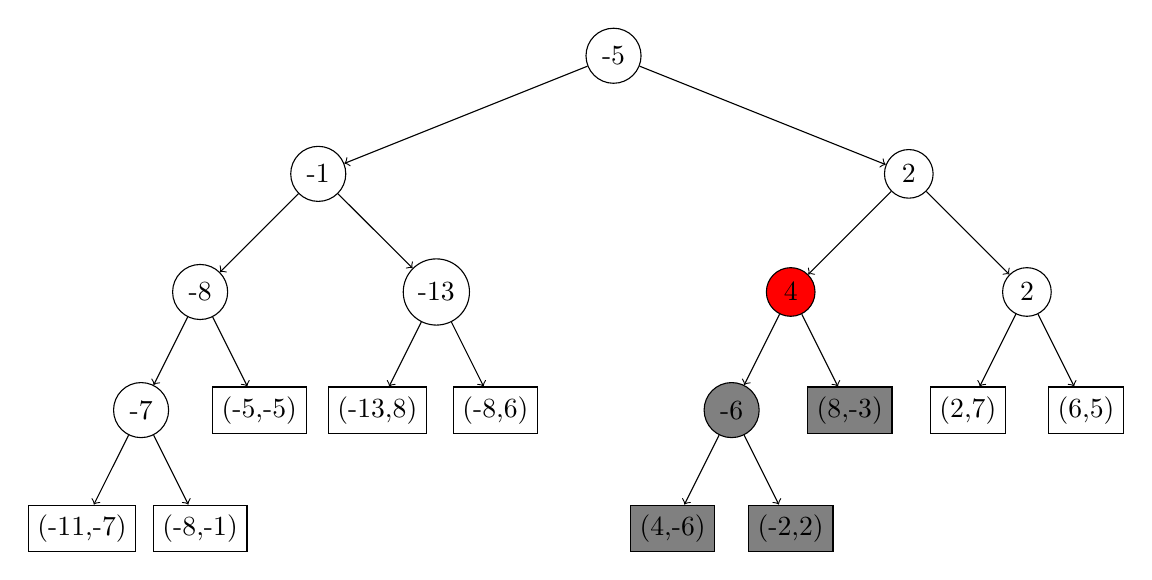
\begin{tikzpicture}[nodes={draw, circle}, ->]
    % Tree structure
 \node{-5}
    child { node {-1} 
        child { node {-8}
            child{ node{-7}
                child{ node[rectangle]{(-11,-7)}}
                child{ node[rectangle]{(-8,-1)}}
            }
            child { node[rectangle]{(-5,-5)}}
        }
        child [missing]
        child { node {-13}
            child { node[rectangle]{(-13,8)}}
            child { node[rectangle]{(-8,6)}}
        }
    }
    child [missing]
    child [missing]
    child [missing]
    child [missing]
    child { node {2} 
        child { node[fill=red]{4}
            child{node[fill=gray]{-6}
                child {node[rectangle, fill=gray]{(4,-6)}  }
                child {node[rectangle ,fill=gray]{(-2,2)}  }
            }
            child{node[rectangle, fill=gray]{(8,-3)}}
        }
        child [missing]
        child { node{2}
            child{node[rectangle]{(2,7)}}
            child{node[rectangle]{(6,5)}}
        }
    };
\end{tikzpicture}


\clearpage

Sejam os pontos da Figura 3, os pontos, segue a construção da árvore.
Temos $P_{ord(x)}$ = $(-13,8), (-11,-7), (-8,6), (-8,-1), (-5,5), (-2, 2), (2,7), (4,-6),(6,5),(8,-3)$.

Criamos um nó raiz com o valor $-5$, dividimos o conjunto de pontos em dois subconjuntos: $P_1$ 
com os pontos com $x \leq -5$ e $P_2$ com os pontos $x > -5$.
Criamos dois nós: $v_{esquerda}$ e $v_{direita}$, e associamos os conjuntos $P_1$ e $P_2$ nas chamadas
recursivas.

A área do nó raiz é calculada como: 
$ -13 \leq x \leq 8 $ e $ -7 \leq y \leq 8$. 

\begin{figure}[H]
    \caption{\label{fig:Fig_5} — Seja}
 \begin{center}
  \begin{tikzpicture}[x=0.25cm,y=0.25cm]
%   \draw[gray!30] (-15,-12) grid[xstep=1, ystep=1]  (15,12);
  \draw[-stealth] (-15,0)--(15,0) node[right]{x}; % x axis
  \draw[-stealth] (0,-12)--(0,12) node[above]{y}; % y axis

\draw[red] (-5,12)--(-5,-12); % y axis

  \fill (-13,8)  circle[radius=2pt] ;
  \fill (-8,6)  circle[radius=2pt] ;
  \fill (-2,2)  circle[radius=2pt] ;
  \fill (-8,-1)  circle[radius=2pt];
  \fill (-11, -7)  circle[radius=2pt];
  \fill (-5,-5)  circle[radius=2pt] node[anchor=north east]{(-5)};
  \fill (2,7)  circle[radius=2pt] ;
  \fill (6,5)  circle[radius=2pt] ;
  \fill (8,-3)  circle[radius=2pt];
  \fill (4,-6)  circle[radius=2pt];
\end{tikzpicture}
     
 \end{center}
  
\end{figure}

E agora repete-se o procedimento para os subconjuntos $P_1$ e $P_2$.
Para os pontos de $P_1$, como a profundidade é ímpar, agora considera uma $y$-ordenação e calcula-se a mediana:
Fazemos uma $y$-ordenação pelos pontos e obtemos a seguinte ordenação:
$P_{1 ordenado(y)}$
\[
    (-11,7), (-5,-5), (-8,-1), (-8,6), (-13,8)
\]

Temos que a mediana é $-1$ cria-se nó com o valor $-1$. Dividimos o conjunto de 
pontos em $P_1 \leftarrow (-11,7), (-5,-5), (-8,-1) $ e $P_2 \leftarrow (-8,6), (-13,8)$.

Sabemos que o eixo foi cortado em $-5$ em $x$.
Calcularemos a área do $nó_{-1}$
\[
    -11 \leq x < -5 \textmd{; e } -5 \leq y < 8
\] 

\begin{tikzpicture}[x=0.25cm,y=0.25cm]
%   \draw[gray!30] (-15,-12) grid[xstep=1, ystep=1]  (15,12);
  \draw[-stealth] (-15,0)--(15,0) node[right]{x}; % x axis
  \draw[-stealth] (0,-12)--(0,12) node[above]{y}; % y axis
  \draw[red] (-5,12)--(-5,-12); % y axis
  \draw[green] (-15,-1)--(-5,-1); % y axis
  \fill (-13,8)  circle[radius=2pt] ;
  \fill (-8,6)  circle[radius=2pt] ;
  \fill (-2,2)  circle[radius=2pt] ;
  \fill (-8,-1)  circle[radius=2pt] node[anchor=north east]{(-1)};
  \fill (-11, -7)  circle[radius=2pt];
  \fill (-5,-5)  circle[radius=2pt] ;
  \fill (2,7)  circle[radius=2pt] ;
  \fill (6,5)  circle[radius=2pt] ;
  \fill (8,-3)  circle[radius=2pt];
  \fill (4,-6)  circle[radius=2pt];
\end{tikzpicture}

Repete-se recursivamente o procedimento até o conjunto $P$ na chamada \Call{ConstróiÁrvore2D}{$P$, $prof$}
contiver somente um ponto. Cria-se então um nó folha, contendo como valor o ponto $p$.

A figura a seguir é a representação dos pontos no plano com os eixos de corte para a construção da 
árvore 2D.

\begin{tikzpicture}[x=0.5cm,y=0.5cm]
%   \draw[gray!30] (-15,-12) grid[xstep=1, ystep=1]  (15,12);
  \draw[-stealth] (-15,0)--(15,0) node[right]{x}; % x axis
  \draw[-stealth] (0,-12)--(0,12) node[above]{y}; % y axis
  \draw[gray] (-5,12)--(-5,-12); % y axis
  \draw[gray] (-15,-1)--(-5,-1); % y axis
  \draw[gray] (15,2)--(-5,2); % y axis
  \draw[gray] (-8,-1)--(-8,-12); % y axis
  \draw[gray] (-13,-1)--(-13,12); % y axis
  \draw[gray] (4,2)--(4,-12); % y axis
  \draw[gray] (2,2)--(2,12); % y axis
  
  \draw[gray] (-15,-7)--(-8,-7); % y axis
  \draw[gray] (4,-6)--(15,-6); % y axis
  
  \fill (-13,8)  circle[radius=2pt]node[anchor=north east]{(-13)};
  \fill (-8,6)  circle[radius=2pt] ;
  \fill (-2,2)  circle[radius=2pt] node[anchor=north east]{(2)};
  \fill (-8,-1)  circle[radius=2pt] node[anchor=north east]{(-8)};
  \fill (-11, -7)  circle[radius=2pt];
  \fill (-5,-5)  circle[radius=2pt] node[anchor=north east]{(-5)} ;
  \fill (2,7)  circle[radius=2pt] ;
  \fill (6,5)  circle[radius=2pt] ;
  \fill (8,-3)  circle[radius=2pt];
  \fill (4,-6)  circle[radius=2pt] node[anchor=north east]{(4)};
\end{tikzpicture}


\clearpage


\subsection{Consulta}
Uma consulta 2-dimensional em $P$ é uma busca de quais pontos de $P$ estão entre um retângulo de consulta
\([x,x']  \times  [y,y']\) que chamaremos de janela. Um ponto $p:= (p_x, p_y)$ está dentro de um
retângulo de busca se e somente se: $p_x \in [x, x'] \textrm{ e } p_y \in [y, y']$.

Podemos dizer que uma consulta 2-dimensional é composta de duas sub-consultas 1-dimensional: uma no
eixo \(x\) de um dos pontos e uma consulta no eixo \(y\).

\begin{figure}[htb]
    \caption{\label{fig:Fig_2} - Consulta 2D}
    \begin{center}
        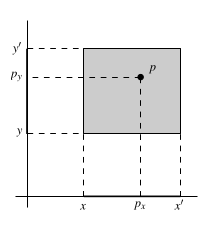
\includegraphics{images/search_range.png}
    \end{center}
\end{figure}


Denotaremos esta área de um nó \(v\) como \(região(v)\). Portanto, o algoritmo buscará pela subárvore
com raiz \(v\) somente se o retângulo de busca intersectar a \(região(v)\).

Seja $P_v$ o conjunto de pontos em folhas alcançáveis a partir de $v$.
Vamos definir a $região(v)$. Seja $P_v$ o conjunto de pontos folhas da árvore alcançáveis a partir de $v$.
Então, a $região(v)$, que é um retângulo no plano, pode ser definida através do intervalo:
\[
 \mbox{
    região(v)=  \begin{cases} min(p_x) \leq x \leq max(p_x) \\ min(p_y) \leq y \leq max(p_y) \end{cases} 
 }
\]

Por exemplo, na figura da árvore 2D anterior, a área do $nó_4$ que guarda o valor 4 
\[
\mbox{
    área_4 =  \begin{cases} -2 \leq x \leq 8 \\ -6 \leq y \leq 2 \end{cases} 
}
\]

Dada uma janela, algoritmo de busca funciona descendo a árvore, mas visitando somente os nós $v$ cuja
\(região(v)\) intersecta a janela. Quando uma \(região(v)\) está contida na janela de busca devolvemos
todos os pontos na subárvore enraizada em $v$. No caso em que chegamos em um nó folha, temos 
que verificar se o nó está dentro da janela, se estiver, devolvê-lo.

\begin{figure}[H]
    \caption{\label{fig:Fig_3} - Em vermelho a área do $nó_4$ e em verde a área do retângulo de consulta}
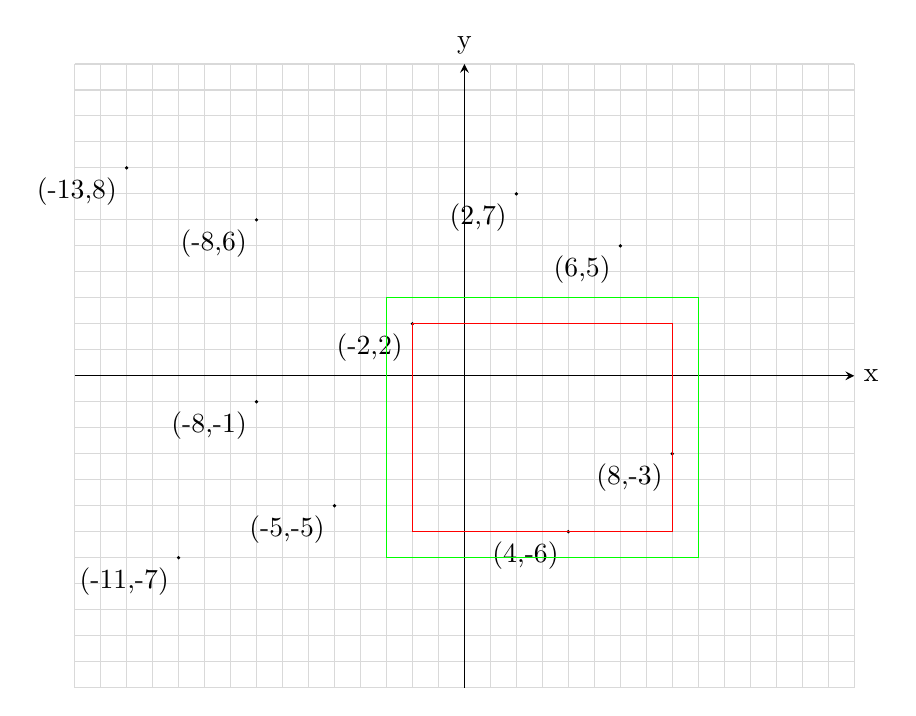
\begin{tikzpicture}[scale=0.33]
  \draw[gray!30] (-15,-12) grid[xstep=1, ystep=1]  (15,12);
  \draw[-stealth] (-15,0)--(15,0) node[right]{x}; % x axis
  \draw[-stealth] (0,-12)--(0,12) node[above]{y}; % y axis


  \fill (-13,8)  circle[radius=2pt] node[anchor=north east]{(-13,8)};
  \fill (-8,6)  circle[radius=2pt] node[anchor=north east]{(-8,6)};
  \fill (-2,2)  circle[radius=2pt] node[anchor=north east]{(-2,2)};
  \fill (-8,-1)  circle[radius=2pt] node[anchor=north east]{(-8,-1)};
  \fill (-11, -7)  circle[radius=2pt] node[anchor=north east]{(-11,-7)};
  \fill (-5,-5)  circle[radius=2pt] node[anchor=north east]{(-5,-5)};
  \fill (2,7)  circle[radius=2pt] node[anchor=north east]{(2,7)};
  \fill (6,5)  circle[radius=2pt] node[anchor=north east]{(6,5)};
  \fill (8,-3)  circle[radius=2pt] node[anchor=north east]{(8,-3)};
  \fill (4,-6)  circle[radius=2pt] node[anchor=north east]{(4,-6)};
  \draw[draw=red] (-2,-6) rectangle (8,2);
  \draw[draw=green] (-3,-7) rectangle (9,3);

\end{tikzpicture}
\end{figure}

Segue o algoritmo que recebe como parâmetros a raiz de uma árvore 2D e uma janela R.
Usamos uma chamada \Call{ReportaSubárvore}{$v$} que atravessa a árvore do nó \(v\) e retorna
todos os pontos nas suas folhas. Segue como notação \(filho_{esq}(v)\) sendo o filho esquerda e
\(filho_{dir}(v)\) o filho direita do nó \(v\).


\begin{algorithm}[H]
    \caption{A função \Call{ConsultaEmÁrvore2D}{$v$, $R$} recebe como parâmetro um nó e uma 
    janela.
     E devolve todos os pontos dentro de R.}
    \begin{algorithmic}[1]
    \Function{ConsultaEmÁrvore2D}{$v$, $R$}
        \If{v é folha}
        \Return  $v$ se estiver dentro da $R$
        \Else
            \If{$região(filho_{esq}(v))$ está contido na $R$}
            \State \Return \Call{ReportaSubárvore}{$filho_{esq}(v)$}
            \Else
                \If{$região(filho_{esquerda}(v))$ intersecta $consulta$}
                \State \Return \Call{ConsultaEmÁrvore2D}{$filho_{esq}(v)$, $consulta$}
                \EndIf
            \EndIf
            \If{$região(filho_{dir}(v))$ está contido na $R$}
                \State \Call{ConsultaEmÁrvore2D}{$filho_{dir}(v)$, $R$}
            \Else
                \If{$região(filho_{dir}(v))$ intersecta $R$}
                \State \Return \Call{ConsultaEmÁrvore2D}{$filho_{dir}(v)$, $R$}
                \EndIf
            \EndIf
        \EndIf
    \EndFunction
    \end{algorithmic}
\end{algorithm}

Para realizarmos uma busca na árvore construída, com uma consulta $ -3 \leq x \leq 9 $ e $-7 \leq y < 3$.
Iniciamos no nó $-5$. Como o nó não é folha, checamos se a área do filho à esquerda esta dentro da consulta.
O $nó_{-1}$ tem área $ -13 \leq x \leq -5 $ e  $ -7 \leq y \leq 8$, logo a área não está contida 
na consulta.

A área dos nós $nó_2$ e $nó_{-1}$ intersectam a consulta, então procedemos chamando
\Call{BuscaEmArvore}{$nó_{-1}$, consulta} e \Call{BuscaEmArvore}{$nó_{2}$, consulta}.

O $nó_{2}$, o $filho_{esquerda}$ é o $nó_4$, que está contido na área da consulta e portanto todos
os pontos folha são retornados.

\subsection{Otimização}
O algoritmo de construção como descrito realiza $log_n$ ordenações para a construção da árvore.
Uma otimização para o algoritmo de construção da árvore KD é realizar apenas $d$ ordenações, onde $d$
é o número de dimensões da árvore KD.
Para isto é preciso ordenar os pontos antes do inicio da construção da árvore e durante a troca de eixo
da árvore, é checar quais pontos no nó pai foram removidos e desconsiderá-los no eixo atual.

A Figura 5 corresponde a uma figura gerada por nossas implementações da árvore 2D. Como esperado, os
pontos dentro de uma janela foram retornados.
\begin{figure}[H][scale=0.5]
    \caption{\label{fig:Fig_54} — Resultados de busca com Arvore2D}
    \begin{center}
        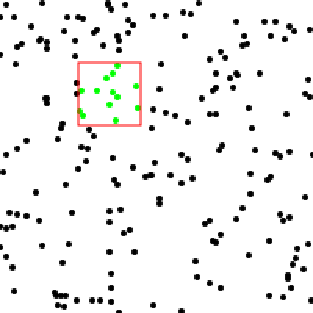
\includegraphics{images/points.pdf}
    \end{center}
\end{figure}
\clearpage



% ----------------------------------------------------------
\section{Árvore de Alcance}
% ----------------------------------------------------------

Uma árvore de alcance é  uma árvore binária onde cada nó não folha é um ponto $k$-dimensional
onde guarda um valor $v$ em uma dimensão $d$ e uma árvore binária auxiliar $\tau$. Para cada $k$-dimensão
existirá uma árvore auxiliar $\tau$ para cada dimensão.

\begin{figure}[htb]
    \caption{\label{fig:Fig_26} — Arvore de Alcance 2D}
    \begin{center}
        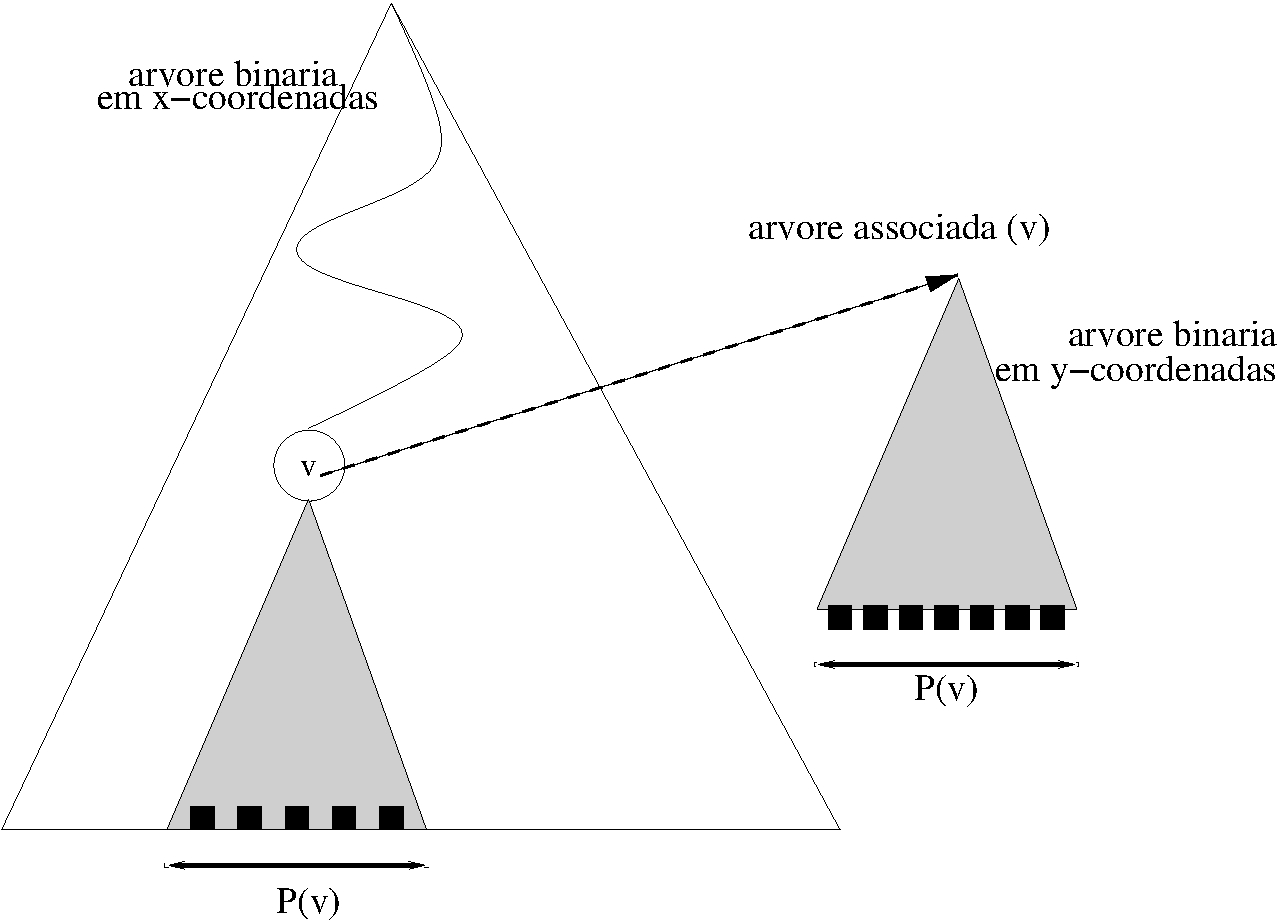
\includegraphics[scale=0.5]{images/range_tree1.pdf}
    \end{center}
\end{figure}

\subsection{Árvore de Alcance 2D}

Uma árvore de alcance 2D é uma versão de duas dimensões para a árvores de alcance. A construção considera
um dado conjunto de pontos $P$ e pode ser feita da seguinte forma:
Temos os pontos da forma $p = (p_x, p_y)$. Ao iniciar a construção, fixamos o eixo $x$;
Construímos uma árvore binária balanceada considerando os valores na $x$-coordenada dos pontos $P$;
Para cada nó não folha $v$ construiremos uma árvore auxiliar $\tau$ com todos os pontos alcançáveis 
a partir de $v$; Esta árvore será construída considerando os valores da $y$-coordenada. Associamos 
$\tau$ ao nó $v$; Os nós folhas por sua vez guardarão os pontos em si.

Considere o seguinte conjunto de pontos.
\begin{figure}[H]

\begin{tikzpicture}[scale=0.5]
  \draw[gray!30] (-15,-12) grid[xstep=1, ystep=1]  (15,12);
  \draw[-stealth] (-15,0)--(15,0) node[right]{x}; % x axis
  \draw[-stealth] (0,-12)--(0,12) node[above]{y}; % y axis


  \fill (15,3)  circle[radius=3pt] node[anchor=north east]{(15,3)};
  \fill (-4,5)  circle[radius=3pt] node[anchor=north east]{(-4,5)};
  \fill (-6,2)  circle[radius=3pt] node[anchor=south west]{(-6,2)};
  \fill (-2,-7)  circle[radius=3pt] node[anchor=north east]{(-2,-7)};
  \fill (3,-9)  circle[radius=3pt] node[anchor=north east]{(3,-9)};
  \fill (0,10)  circle[radius=3pt] node[anchor=north east]{(0,10)};
  \fill (7,-11)  circle[radius=3pt] node[anchor=north east]{(7,-11)};
  \fill (-7,-3)  circle[radius=3pt] node[anchor=north west]{(-7,-3)};
  \fill (-8,8)  circle[radius=3pt] node[anchor=sul east]{(-8,8)};
  \fill (4,2)  circle[radius=3pt] node[anchor=north west]{(4,2)};

\end{tikzpicture}

\end{figure}
% imagem

% arvore [(15,3),(-4, 5),(2,2),(-2,-2),(3,1),(0,0),(4,-2),(3,3),(1,1),(1,2)]
Para construir uma árvore binária balanceada é necessário que os pontos estejam ordenados.
Ordenamos os pontos $P$ pela $x$-coordenada inicialmente. Escolhemos o ponto médio $x_{mediana}$ guardamos
em $v$ e criamos dois subconjuntos $P_1$ e $P_2$ tal que:

    $P_1 = \{p \in P : p_x \leq x_{mediana}\}$ e $P_2 = \{p \in P : p_x > x_{mediana}\}$.

Criamos uma árvore binária balanceada $\tau$ em $P$ considerando o valor da $y$-coordenada dos pontos
de $P$.
A árvore associada correspondente e o pseudocódigo sao dados em seguida.
\begin{figure}[htb]
    \caption{\label{fig:Fig_16} - Consulta 2D}
    \begin{center}
        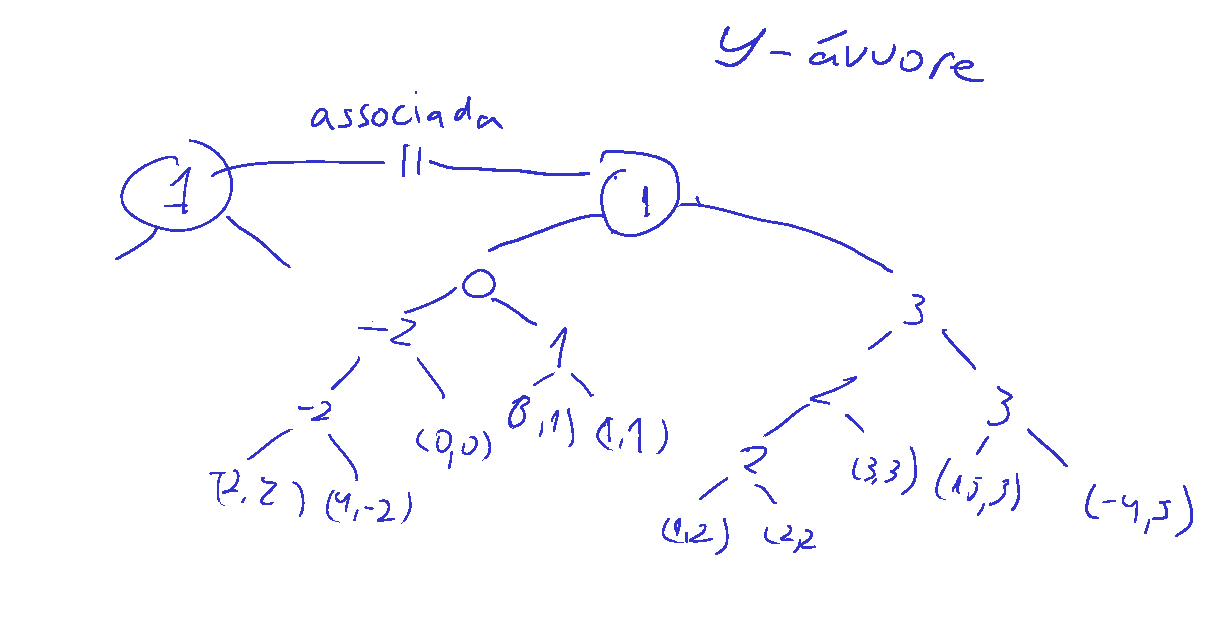
\includegraphics[width=\textwidth]{images/assoc_tree.pdf}
    \end{center}
\end{figure}


\begin{algorithm}[H]
    \caption{A função \Call{ConstróiÁrvoreAlcance2D}{$R$} Recebe como entrada um conjunto de pontos 
    $P$ e devolve o nó raiz de uma árvore de alcance 2-$dimensional$.}
    \begin{algorithmic}[1]
    \Function{ConstróiArvoreAlcance2D}{ $R$}
        \State Constrói a árvore binária associada: Constrói uma árvore binária $\tau_{associada}$ no conjunto de pontos
        $P_y$  de $y$-coordenadas dos pontos em $P$. Nas folhas de de $\tau_{associada}$ guardaremos
        os pontos em si.
        \If{$P$ contem apenas um ponto}
            \State Cria um nó $v$ guardando o ponto e fazemos $\tau_{associada}$ a árvore associada 
            à $v$.
        \Else
            \State Dividimos $P$ em dois subconjuntos. $P_1$ contem os pontos com a $x$-coordenada $\leq$
            que $x_{mediana}$, e $P_2$ contém os pontos com $x$-coordenada $>$ que $x_{mediana}$.
            \State $v_{esq} \leftarrow $ \Call{ConstróiArvoreAlcance2D}{$P_1$}
            \State $v_{dir} \leftarrow $ \Call{ConstróiArvoreAlcance2D}{$P_2$}
            \State Criamos um nó $v$ guardando $x_{mediana}$, fazemos $v_{esq}$ e $v_{dir}$ filhos de 
            $v$ e associamos $\tau_{associada}$ a estrutura associada de $v$.
        \EndIf
    \Return $v$
    \EndFunction
    \end{algorithmic}
\end{algorithm}

%pseudo codigo

Sejam os pontos da figura ordenados pelo eixo $x$ =

$(-4, 5),(-2,-2),(0,0),(1,1),(1,2),(2,2), (3,1),(3,3),(4,-2),(15,3)$

Criamos um nó raiz com o valor da $x_{mediana} = 1$. Dividindo o conjunto de pontos em dois subconjuntos:
$P_1$ com os pontos $x\leq 1$ e $P_2$ com os valores $x > 1$.
Fazemos uma $y$-ordenação nos pontos e construiremos uma árvore binária balanceada considerando os 
valores dos pontos pelo eixo $y$ e associaremos a árvore resultante ao $nó_1$.


Criamos dois nós: $v_{esquerda}$ e $v_{direita}$ e associamos os conjuntos $P_1$ e $P_2$ nas chamadas
recursivas.

Agora repete-se o procedimento para os subconjuntos $P_1$ e $P_2$.
Para os pontos de $P_1$, temos o valor $x_{mediana} = 2$. Associaremos a este nó a árvore binária auxiliar
construída com os pontos fixando o eixo $y$.
% arvore com nó 1 e nó 2, nó_2 indicando a árvore associada construida 

Repete-se recursivamente \Call{ConstróiArvoreAlcance2D}{$P$} até o conjunto $P$ contiver somente um ponto.
Cria-se um nó folha contendo como valor o ponto $p$ em ambas as árvores.

A figura a seguir é a representação dos pontos no plano em uma árvore de alcance.

\begin{figure}[htb]
    \caption{\label{fig:Fig_16} - Consulta 2D}
    \begin{center}
        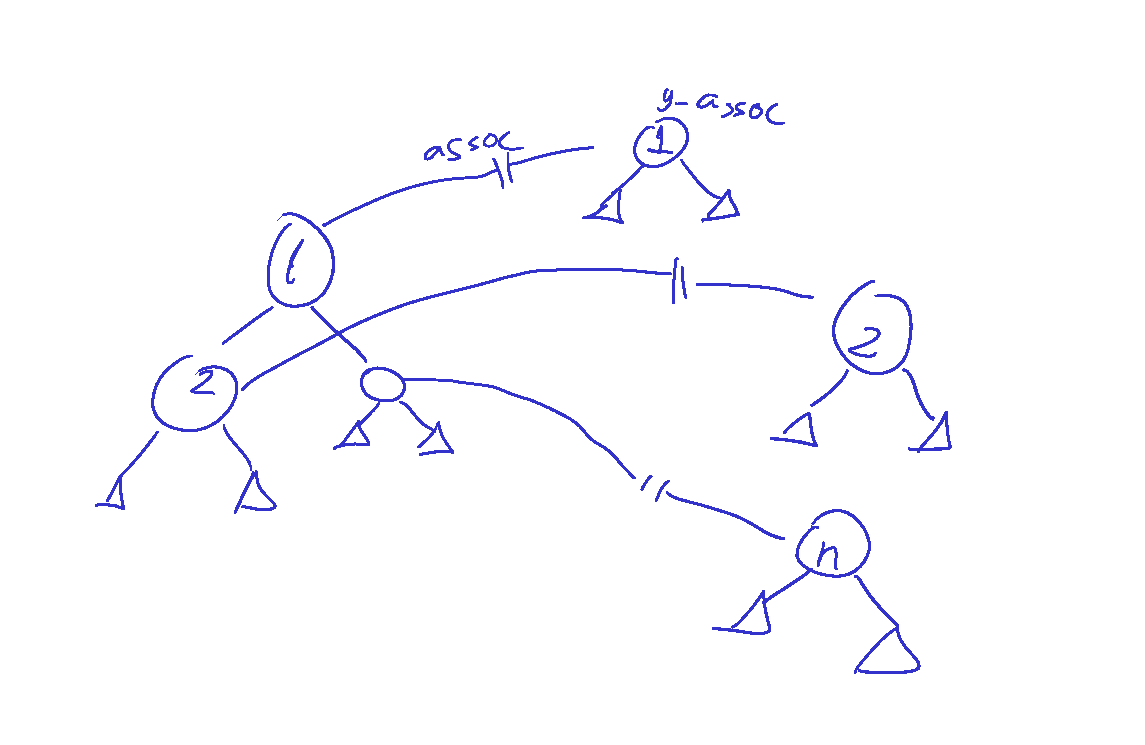
\includegraphics[width=\textwidth]{images/range_assoc2.pdf}
    \end{center}
\end{figure}

\subsection{Consulta}

Uma consulta 2-dimensional em $P$ é uma busca de quais pontos de $P$ estão entre uma janela de consulta
$[x, x'] \times [y, y']$. Um ponto $p = (p_x, p_y)$ está dentro de um retângulo de consulta se e somente
se $p_x \in [x, x']$ e $p_y \in [y, y']$. \cite{cg_rt1}

Uma consulta em uma árvore de alcance é a combinação de $n$ consultas em árvore, onde $n$ é a dimensão
da árvore de alcance.
Na árvore de alcance 2-dimensional temos uma consulta no eixo $x$ seguida por uma consulta na arvore 
auxiliar $\tau$ que foi construída considerando $y$-coordenada.

A consulta com janela, consistirá portanto na união de duas consultas de intervalo unidimensional em
árvore.

\subsection{Consulta de intervalo unidimensional}

Seja uma árvore binária balanceada $\Gamma$. Uma consulta de intervalo em $\Gamma$ é tal que queremos
todos os nós folhas de $\Gamma$ cujo valor esteja dentro do intervalo consultado $[x, x']$.

Dado o intervalo da consulta $R = [x , x']$ e a raiz de $\Gamma$ sobre realizaremos o seguinte algoritmo:
Inicialmente precisamos encontrar o nó que está dentro da consulta. Chamaremos este nó de $nó_{corte}$.
Para encontrar o $nó_{corte}$ faremos uma consulta simples que a partir da raiz $v$ checaremos se $v$
está dentro do intervalo buscado. Se estiver será nosso $no_{corte}$. Do contrario checaremos se $v > x'$
caso seja, $v$ é maior que o maior valor da consulta, então faremos recursivamente a busca por $no_{corte}$
passando o $nó_{esquerda}$ de $v$. Caso $v \leq x$ realizaremos a consulta por $nó_{corte}$ recursivamente
em $no_{direita}$ de $v$.

Munidos de $nó_{corte}$, faremos a consulta para retornar todos os pontos contidos dentro de $R$ na árvore
$\Gamma$.
A partir de $nó_{corte}$, queremos recursivamente buscar os pontos que são menores que $nó_{corte}$ porem
ainda dentro da consulta, e similarmente, os pontos maiores que $nó_{corte}$ ainda dentro do intervalo.
Assim como buscar os pontos maiores que $nó_{corte}$ e dentro da consulta. \cite{cg_search1}

Para buscarmos os valores menores que $nó_{corte}$ iremos realizar uma consulta em profundidade considerando
os nós não folha à esquerda a partir de $nó_{corte}$ checando se valor do nó $v$ é $v > x$. 
Quando essa condição não for mais atendida, ou seja, $nó \leq x$  isso significa que já não mais está
dentro da consulta. Neste ponto checaremos se o nó à direita está dentro da consulta. Caso esteja reportamos.
Durante a busca em profundidade todos os pontos que atendem $v > x$, reportamos a subárvore à direita
deste nó, ou seja, temos certeza que os valores desta subárvore está dentro do intervalo consultado.

A mesma busca em profundidade será realizada para os valores maiores que $nó_{corte}$, checando se 
o $nó < x'$ e reportando todas as subárvores à esquerda que atendem essa condição. E no caso onde essa
condição seja quebrada checando o nó à esquerda e reportando caso dentro do intervalo.

A condição de parada dessa busca em profundidade é caso seja um nó folha, e caso seja, deve se checar
se está dentro do intervalo, caso esteja reporta-o.

Em seguida temos o pseudocódigo para buscar o $nó_{corte}$ e para consulta unidimensional.

\begin{algorithm}[H]
    \caption{A função \Call{EncontraNóCorte}{$v$, $R$} recebe como parâmetro um nó e uma 
    janela.
     E devolve o primeiro ponto dentro janela de consulta.}
    \begin{algorithmic}[1]
    \Function{EncontraNóCorte}{$v$, $R$}
        \While{$v$ não é folha}
        \If{$v \in R$ } 
            \Return $v$
        \Else
            \If{$v > R$ }
                \State $v \leftarrow v_{direita}$ 
            \Else
                \State $v \leftarrow v_{left}$
            \EndIf
        \EndIf
    \EndFunction
    \end{algorithmic}
\end{algorithm}
\clearpage


\begin{algorithm}[H]
    \caption{A função \Call{Busca1DEmAlcance}{$v$, $R$} recebe um nó e uma consulta e retorna todos
    os pontos dentro da consulta.}
    \begin{algorithmic}[1]
    \Function{Busca1DEmAlcance}{$v_{corte}$, $R$}
        \If{$v_{corte}$ é folha}
            \If{$v_{corte} \in R$}
                \State Reporta ponto $v_{corte}$
            \EndIf
        \Else
            \State $v \leftarrow filho_{esq}(v_{corte})$
            \While{$v$ não for folha}
                \If{$v > R$}
                    \State \Call{ReportaSubárvore}{$v$}
                    \State $v \leftarrow filho_{esq}(v)$
                \Else
                    \State $v \leftarrow filho_{esq}(v)$
                \EndIf
            \EndWhile
            \If{$v$ é ponto e $v \in R$}
                \State Reporta ponto $v$
            \EndIf


            \State $v \leftarrow filho_{dir}(v_{corte})$
            \While{$v$ não for folha}
                \If{$v < R$}
                    \State \Call{ReportaSubárvore}{$v$}
                    \State $v \leftarrow filho_{dir}(v)$
                \Else
                    \State $v \leftarrow filho_{dir}(v)$
                \EndIf
            \EndWhile
            \If{$v$ é ponto e $v \in R$}
                \State Reporta ponto $v$
            \EndIf
        \Endif
    \EndFunction
    \end{algorithmic}
\end{algorithm}
\clearpage


Sejam os pontos da Figura 3, os pontos, segue a construção da árvore.
Temos $P_{ord(x)}$ = $-4, -2, 0, 1, 1, 2, 3, 3, 4, 15$
Na figura 5 temos a árvore construída em relação a coordenada $x$.
Iremos fazer uma consulta de intervalo nesta arvore inicialmente.
Seja o intervalo de consulta $R = [-8, 2]$

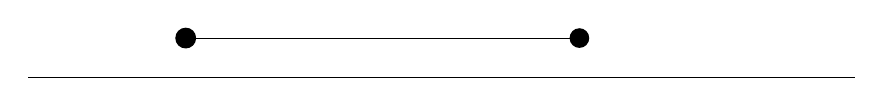
\begin{tikzpicture}[scale=0.5]
\draw (-12,0)-- (9,0); %Axis

\draw (-8,1) -- (2,1);
\draw[fill=black] (-8,1) circle (0.25);
\fill (2,1) circle (0.25);
\end{tikzpicture}

Começamos pelo nó raiz com valor $1$. A condição $-8 \leq 1 \leq 2$ é verdadeira. Portanto $nó_{1}$
será nosso $nó_{corte}$.
A partir dele, primeiramente iremos obter os nós $v$ tal que $v \leq 1$. Começamos a busca em profundidade:
o nó a esquerda de $nó_{1}$ é $no_{0}$. Reportamos a subárvore à direita $nó_{0}$.
O valor $0$ ainda mantém $-8 \leq 0$, e, portanto, continuamos a busca em profundidade. 
Agora temos o $nó_{-2}$. Por sua vez, satisfaz  $-2 \leq -8$, reportamos a subárvore à direita. A busca
em profundidade continuará até o $no_{-4}$, que satisfaz a consulta porém é o ultimo nó não folha. Reportamos
a subárvore à direita e saímos. Checando se o nó folha $(-4)$ esta dentro da consulta, e está.
Realizaremos o mesmo procedimento, porem, á partir de $nó_{corte}$ iremos realizar busca em profundidade
à pela direita considerando se o valor do nó é $nó \leq 2$.

Por fim teremos os nós $(-4, -2, 0, 1, 1, 2)$.

\subsection{Consulta Bidimensional}

Para realizar uma consulta bidimensional, iremos realizar uma consulta de intervalos unidimensional para
cada dimensão. 
Iremos para cada nó visitado que está dentro da janela de consulta, será feita outra busca unidimensional
na árvore $\tau$ associada ao nó.
Segue pseudocódigo pra consulta bidimensional:

\begin{algorithm}[H]
    \caption{A função \Call{Busca2DEmAlcance}{$v$, $R$} recebe um nó e uma consulta e retorna todos
    os pontos dentro da consulta.}
    \begin{algorithmic}[1]
    \Function{Busca2DEmAlcance}{$v_{corte}$, $R : [x,x'] \times [y,y']$}
        \If{$v_{corte}$ é folha}
            \If{$v_{corte} \in R_x$}
                \State Reporta ponto $v_{corte}$
            \EndIf
        \Else
            \State $v \leftarrow filho_{esq}(v_{corte})$
            \While{$v$ não for folha}
                \If{$v > R_x$}
                    \State Reporta pontos \Call{Busca1DEmAlcance}{$v$, $R_y$}
                    \State $v \leftarrow filho_{esq}(v)$
                \Else
                    \State $v \leftarrow filho_{esq}(v)$
                \EndIf
            \EndWhile
            \If{$v$ é ponto e $v \in R$}
                \State Reporta ponto $v$
            \EndIf


            \State $v \leftarrow filho_{dir}(v_{corte})$
            \While{$v$ não for folha}
                \If{$v < R_x$}
                    \State \Call{ReportaSubárvore}{$v$, $R_y$}
                    \State $v \leftarrow filho_{dir}(v)$
                \Else
                    \State $v \leftarrow filho_{dir}(v)$
                \EndIf
            \EndWhile
            \If{$v$ é ponto e $v \in R$}
                \State Reporta ponto $v$
            \EndIf
        \Endif
    \EndFunction
    \end{algorithmic}
\end{algorithm}
\clearpage

Iremos agora demonstrar uma consulta bidimensional com intervalos $x : [-8, 2]$ e em $y : [-7, 3]$
Iniciamos a busca no nó raiz $nó_{1}$. Temos que inicialmente encontrar o $nó_{corte}$ e $nó_{1}$ 
está dentro da consulta em $[-8, 2]$. 
A partir dele faremos uma busca em profundidade para esquerda e para a direita para encontrar todos 
os valores dentro do intervalo $[-8,2]$. 
Ao invés de retornar a subárvore da direita, iremos fazer uma busca em profundidade na árvore associada
$\tau$ do nó à direita. 
Inicialmente $nó_{1}$, o nó à esquerda $nó_{0}$, está dentro da consulta e portanto realizaremos uma
busca em profundidade na árvore $\tau$ associada $nó_{0}$.




% ----------------------------------------------------------